\begin{question}
\noindent Triangle $T$ has vertices $A(1,1)$, $B(1,3)$ and $C(2,1)$.

\begin{center}
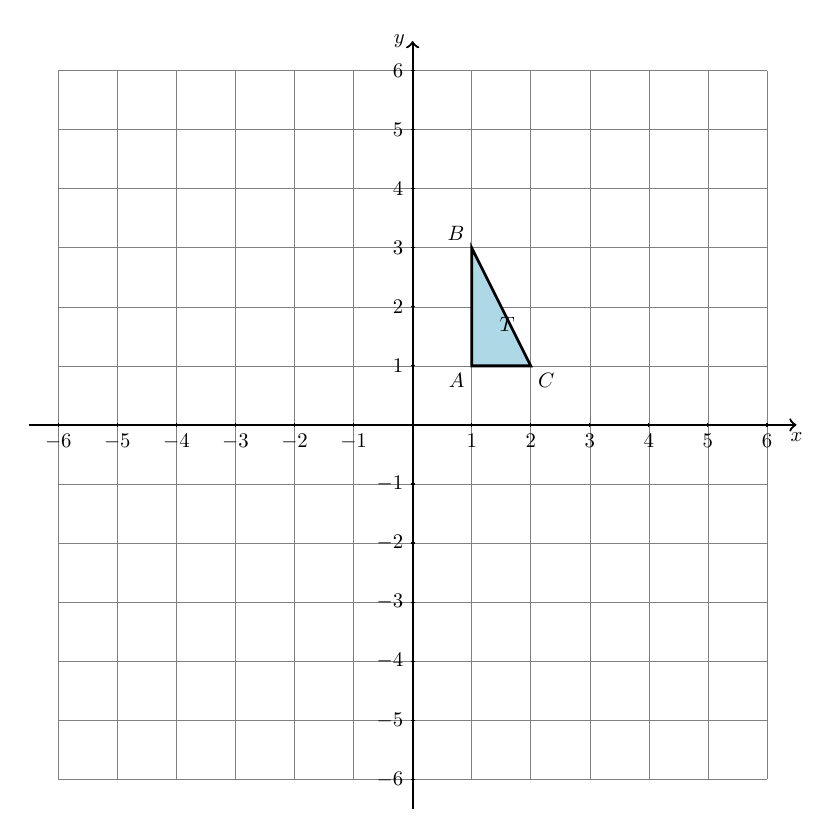
\begin{tikzpicture}[scale=0.75, transform shape]
    \def\axisLimit{6}
    \definecolor{borderColour}{HTML}{000000}
    \definecolor{fillColourT}{HTML}{ADD8E6}

    % Draw grid
    \draw[step=1cm,gray,very thin] (-\axisLimit,-\axisLimit) grid (\axisLimit,\axisLimit);

    % Draw axes
    \draw[thick,->] (-\axisLimit-0.5,0) -- (\axisLimit+0.5,0) node[anchor=north] {$x$};
    \draw[thick,->] (0,-\axisLimit-0.5) -- (0,\axisLimit+0.5) node[anchor=east] {$y$};

    % Label x-axis and y-axis
    \foreach \x in {-\axisLimit,...,-1,1,2,...,\axisLimit}
        \draw (\x cm,1pt) -- (\x cm,-1pt) node[anchor=north] {$\x$};
    \foreach \y in {-\axisLimit,...,-1,1,2,...,\axisLimit}
        \draw (1pt,\y cm) -- (-1pt,\y cm) node[anchor=east] {$\y$};

    % Triangle T: A(1,1), B(1,3), C(2,1)
    \coordinate (A) at (1,1);
    \coordinate (B) at (1,3);
    \coordinate (C) at (2,1);
    \filldraw[fill=fillColourT, draw=borderColour, line width=1pt] (A) -- (B) -- (C) -- cycle;

    \node[below left] at (A) {$A$};
    \node[above left] at (B) {$B$};
    \node[below right] at (C) {$C$};
    \node at (1.6,1.7) {$T$};
\end{tikzpicture}
\end{center}

\noindent Triangle $T$ is first rotated $90^\circ$ clockwise about the origin $(0,0)$ to give triangle $T_1$.

\noindent Triangle $T_1$ is then reflected in the $x$-axis to give triangle $T_2$.

\begin{enumerate}
    \item[(a)] Write down the coordinates of the vertices of triangle $T_2$.

    \vspace{4cm}
    \answerplain{2}

    \item[(b)] Describe \textbf{fully} the \textbf{single} transformation that maps triangle $T$ directly onto triangle $T_2$.\\
    (A description involving two transformations will not gain full credit.)

    \vspace{4cm}
    \answerlines{3}{2}
\end{enumerate}
\end{question}
